\documentclass[french,a4paper,answers,addpoints,12pt]{exam}%
\usepackage[T1]{fontenc}%
\usepackage[utf8]{inputenc}%
\usepackage{lmodern}%
\usepackage{textcomp}%
\usepackage{lastpage}%
\usepackage[width=170mm,left=20mm,top=30mm,bottom=20mm,head=20mm]{geometry}%
\usepackage{qrcode}%
\usepackage{tikz}%
\usepackage{tabularx}%
\usepackage{ragged2e}%
\usepackage{graphicx}%
\newcommand{\class}{Master d'informatique}%
\newcommand{\examunit}{ARES}%
\newcommand{\allowdocuments}{Notes de cours autorisées}%
\newcommand{\examnum}{Première Session}%
\newcommand{\term}{Janvier 2014}%
\newcommand{\examyear}{2017{-}2018}%
\newcommand{\timelimit}{2 Heures}%
\newcommand{\university}{Université Pièrre et Marie Curie}%
\newcommand{\examtitle}{Examen du 15 décembre 2017}%
\usetikzlibrary{positioning}%
\checkboxchar{$\Box$}%
\checkedchar{$\blacksquare$}%
\pagestyle{headandfoot}{ 
\header{ 
}%
\footer{ 
}
}%
%
\begin{document}%
\normalsize%
\headrule%
\lhead{ 

\begin{tikzpicture}[node distance=5mm]%
\node[draw,circle,anchor=west,minimum size=0.5cm,fill=black] (lCircle) {};%
\node[right=of lCircle] (SNL) {Numéro d étudiant};%
\node[draw,right=of SNL,minimum height=1cm,minimum width=4cm] (SNB) {};%
\end{tikzpicture}
}%
\rhead{ 

\begin{tikzpicture}[node distance=5mm]%
\node[draw,circle,anchor=east,minimum size=0.5cm,fill=black] (rCircle) {};%
\node[left=of rCircle] (QR) {\qrcode[version=5, height=1cm]{3012522}};%
\end{tikzpicture}
}%
\lfoot{ 

\begin{tikzpicture}[node distance=5mm]%
\node[draw,circle,anchor=west,minimum size=0.5cm,fill=black] (lCircle) {};%
\end{tikzpicture}
}%
\cfoot{ 
Center Footer
}%
\rfoot{ 

\begin{tikzpicture}[node distance=5mm]%
\node[draw,circle,anchor=east,minimum size=0.5cm,fill=black] (rCircle) {};%
\end{tikzpicture}
}%
\noindent%
\begin{tabularx}{\linewidth}{c X c}%
\centering%
\textbf{\class}&\textbf{Module \examunit}&\textbf{\university}\\%
\textit{\allowdocuments}&\textit{Durée \timelimit}&\textit{Année \examyear}\\%
\end{tabularx}%
\begin{center}%
\vspace*{1em}%
\textbf{\begin{Large}%
\examtitle%
\end{Large}}%
\vspace*{1em}%
\end{center}%
\begin{center}%
\setlength%
\fboxrule{1pt}%
\setlength%
\fboxsep{1em}%
\fbox{ 
\parbox{0.95\textwidth}{ 
\textbf{Important}%
\linebreak%
Cet examen contient \numpages\ pages (cette page incluse) et \numquestions\ questions.Total of points is \numpoints\
                             Rest of introduction. Rest of introduction. Rest of introduction. Rest of introduction. Rest of introduction. Rest of introduction. Rest of introduction. Rest of introduction.
}
}%
\end{center}%


\begin{figure}[h!]%
\centering%
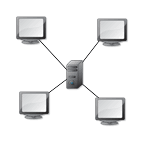
\includegraphics[width=120px]{pstl/figures/type_reseau.png}%
\caption{légende}%
\end{figure}

%
\begin{tabular}{|l|c|r|}%
 col 1 & col 2 & col3 \\%
\hline%
 s     & s     & a    \\%
&&\\%
\end{tabular}%
\linebreak%
\end{document}